\chapter{Разработка программной системы для классификации сигналов фМРТ}


\section{Проектирование программного пакета выполняющего классификацию когнитивных состояний по данным фМРТ на основе анализа межиндивидуальных корреляций}

Для проведения сравнительного анализа различных методов сегментации и классификации было решено использовать гибкую архитектуру типа "Data pipeline". Учитывая значительные затраты времени и ресурсов на использования метода ISC было принято решение реализовать алгоритм на языке Julia\cite{bezanson2017julia}
\begin{figure}%
	\begin{center}
		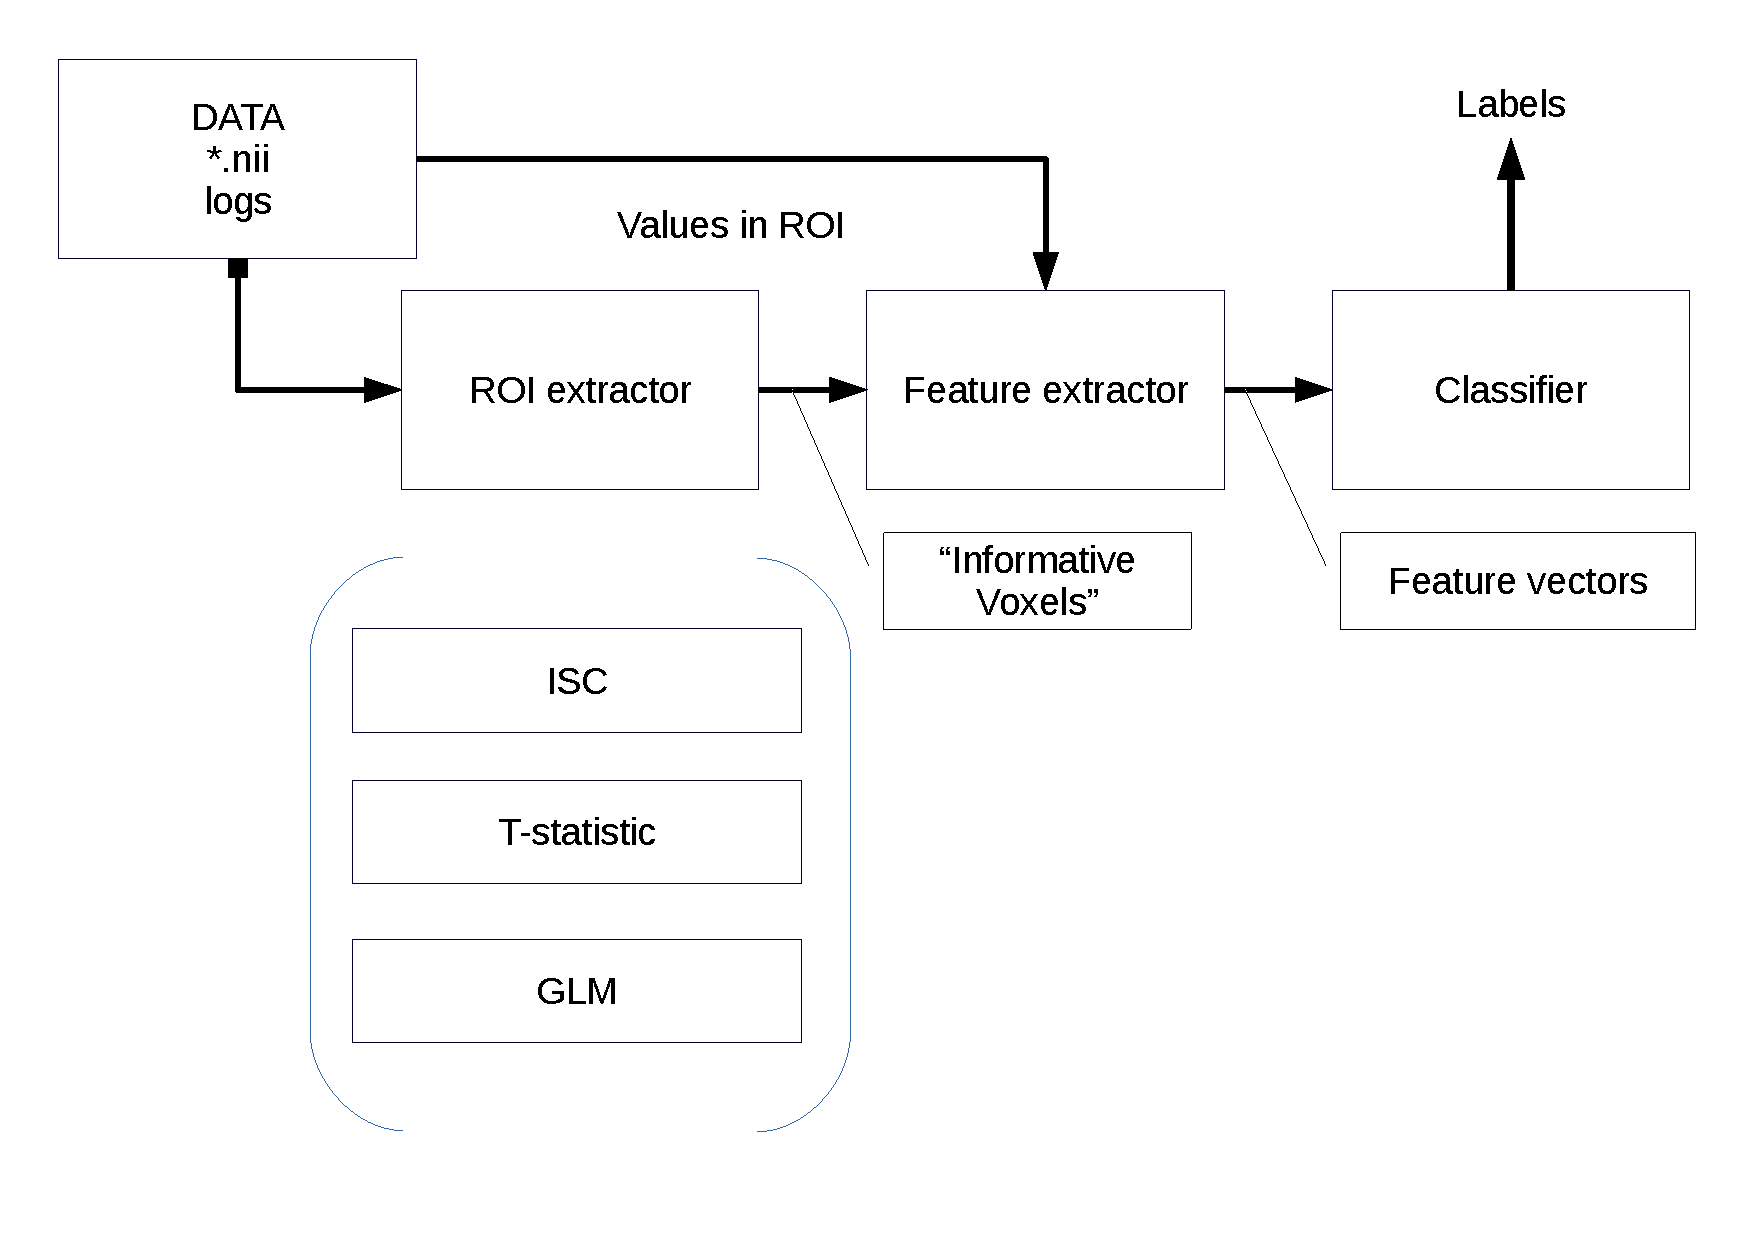
\includegraphics[width=.7\columnwidth]{./img/arch.pdf}%
	\end{center}
	\caption{Архитектура разработанной системы}%
	\label{pic:arch}%
\end{figure}



\section{Программная реализация системы классификации}
\begin{annotation}
	Здесь будет описана реализация
	\begin{compactitem}
		\item алгоритма быстрой загрузки примеров для обучения и кластеризации.
		
	\end{compactitem}

\end{annotation}
В этом разделе обосновывается выбор инструментальных средств; одним из критериев выбора могут быть какие-либо требования к разрабатываемой системе, и если этих требований много, они могут быть выделены в отдельный раздел, или же в приложение. Этот пункт не пишется, если в аналитической главе был раздел, посвященный сравнительному анализу и выбору инструментальных средств.




\section{Состав и структура реализованного программного обеспечения}
\begin{annotation}
	Разработанное приложение является подключаемой библиотекой для использования в среде "интерактивных тетрадей" \texttt{jupyter}. В состав библиотеки входят:
	\begin{compactitem}
		\item Модуль параллельной загрузки/выгрузки примеров/изображений
		\item Модуль кластеризаци, содержащий алогритмы, описанные в части 2.
		\item Модуль классификации, предоставляющий на выбор несколько классификаторов и их входные параметры.
		\item Модуль визуализации для удобного представления данных для последующегог анализа специалистом		
	\end{compactitem}
\end{annotation}

\section{Основные сценарии работы пользователя}
\begin{annotation}
	Подразумевается следующий сценарий работы: пользователь подключатся к серверу интерактивных рабочих тетрадей декларативно описывает свои действия. Сценарий подразумевает загрузку дополнительных обучающих/тестовых выборок для проверки корректности работы алгоритмов.
\end{annotation}

\section{Сравнение реализованного программного обеспечения с существующими аналогами}
\begin{annotation}
	Автор не нашёл аналогов данного приложения по причине низкой востребованности.
\end{annotation}

В сравнении должно быть отражено, чем полученное ПО выгодно (и невыгодно) отличается от прочих ближайших аналогов. Практика показывает, что аналоги есть всегда. А если нет аналогов, значит есть частичные решения, которые реализуют какие-то части функционала вашей системы. Тут тоже может быть относительно много таблиц и графиков.



\section{Выводы}

Следует перечислить, какие практические результаты были получены, а именно: какое программное или иное обеспечение было создано. В число результатов могут входить, например, методики тестирования, тестовые примеры (для проверки корректности/оценки характеристик тех или иных алгоритмов) и др. По каждому результату следует сделать вывод, насколько он отличается от известных промышленных аналогов и исследовательских прототипов.

